\section{Lezione 2016-11-0x}
\subsection{TODO}
% Insert what you need. Any row is associated with the improvment or mistake
% arise. In the first column you can insert what you should resolve or change,
% instead in the second column you may put the section where to apply some
% modification.
\begin{table}[H]
\begin{center}
\begin{tabular}{|p{\textwidth}|c|}
\hline
\multicolumn{1}{|c|}{\textbf{Miglioramento}} & \textbf{Sezione} \\ \hline
\end{tabular}
\end{center}
\caption{Tabella miglioramenti}
\label{tab:tab_todo}
\end{table}

\subsection{Generatore codice intermedio}
Lo scopo del codice intermedio \`e \textbf{facilitare il retargeting}:
riutilizzare i \textit{front-end} esistenti modificando, o creando, un
\textit{back-end} compatibile con la nuova macchina obiettivo. Ovviamente segue
la l'idea di il riutilizzo del codice inserendo uno stato d'astrazione
superiore, ovvero il codice intermedio.

\begin{figure}[H]
  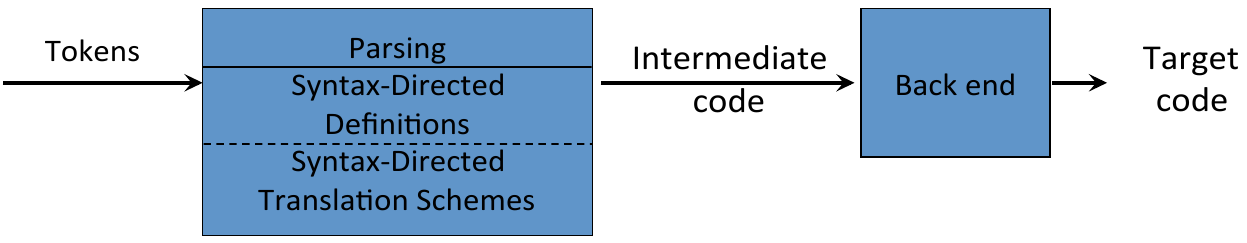
\includegraphics[scale=0.4]{res/image/compiler_backend}
  \caption{Codice intermedio, ponte tra \textit{front-end} e \textit{back-end}}
  \label{img:compiler_backend}
\end{figure}

\`E da specificare che il "codice" intermedio \`e pi\`u la rappresentazione
di come il \textit{front-end} comunica le azioni semantiche al
\textit{back-end} specificate nel sorgente del programma. Possibili
rappresentazioni sono:
\begin{itemize}
\item Rappresentazioni grafiche (es. AST e DAG)
\item Notazioni postfissa (simile alla JVM)
\item \textbf{Three-address code}: $x := y op z$
\item Two-address code ($x := op y$)
\end{itemize}

\subsection{Rappresentazioni grafiche - AST}
Utilizzando la \textit{Syntax-Directed Translation Table} si va a definire,
nelle \textit{semantic rules}, la costruzione dell'AST.
